% ============================ 四、数据审计与探索性分析 ============================
\section{数据审计与探索性分析}

数据审计不是“清洗一下再建模”的例行公事。本题的三处关键设定——\textbf{对数
变换底数}、\textbf{缺失与检出限机制}、\textbf{0--6 分制标定}——若判错，后面三问
的结论会系统性偏移且互相矛盾。本章逐项给出\textbf{可复算}的判定依据。

\subsection{数据结构与对齐}

八份附件的数据形态如表~\ref{tab:data}。需要特别注意两点：其一，\texttt{4.csv}
的 \texttt{beer\_id} 列是\textbf{截断后}的条码——250 行中有 \textbf{213 行}与
\texttt{1.csv} 的同名酒款不一致（例如 \texttt{5413970150111} 被记为
\texttt{5413970000000}），因此\textbf{不能}用 \texttt{beer\_id} 做主键；本文全程
以 \texttt{beer} 编号（1--250）对齐，实测 250 行一一对应。其二，\texttt{2.csv}
与 \texttt{6.csv} 使用\textbf{规范化学名}（\texttt{Acetaldehyde}、
\texttt{Carbon\ disulfide}），而 \texttt{1.csv} 使用转义列名
（\texttt{acetaldehyde}、\texttt{CS2}），二者需建立映射。

\begin{table}[H]
\centering
\caption{附件数据形态与本文用途}
\label{tab:data}
\small
\begin{fittable}
\begin{tabular}{@{}llll@{}}
\toprule
文件 & 规模 & 内容 & 本文用途 \\
\midrule
\texttt{1.csv} & $250\times234$ & 231 个化合物丰度 + 风格标签 & 问题一、三的自变量 \\
\texttt{2.csv} & $231\times231$ & 化合物间皮尔逊相关 & 问题二共表达图；问题一图扩散 \\
\texttt{3.xlsx} & 13 工作表 & 0--6 分制品评卡（含锚点描述） & 感官维度定义与分制依据 \\
\texttt{4.csv} & $250\times52$ & 50 维感官评分（标准化后） & 问题一、三的监督目标 \\
\texttt{5.csv} & $50\times50$ & 感官维度间 Spearman 相关 & 多任务结构证据 \\
\texttt{6.csv} & $44\times50$ & 化学 $\times$ 感官交叉相关 & 问题二独立验证证据 \\
\texttt{7.csv} & $250\times188$ & 186 个评论香气描述符 & 探索性佐证（未入模） \\
\texttt{8.xlsx} & 6 工作表 & 阈值 / 来源 / 校准浓度 / 价格 & OAV 与化学合理性 \\
\bottomrule
\end{tabular}
\end{fittable}
\end{table}

\texttt{2.csv} 的 231 个规范名与 \texttt{1.csv} 的 231 个转义名并非一一可字符串
匹配：其中 11 个存在拼写差异（\texttt{Terpiryl\ acetate}、\texttt{Tobacarol}、
\texttt{Kongol}、\texttt{Epicubenol} 等）。本文用“规范名 $\rightarrow$ 化学名
$\rightarrow$ 原名”三级归一化（小写、去标点、希腊字母展开）配合人工核对，建成
\textbf{231 $\rightarrow$ 231 的双射}，无遗漏、无重复。

\subsection{对数变换底数的判定}\label{sec:logbase}

附件说明称“部分数值为原始浓度经对数变换后的结果（负值对应浓度小于 1）”，但
\textbf{未给出底数}；同时又说明“少量理化参数列保留原始量纲”。这留下两个必须
回答的问题：底数是 10 还是 $e$？哪些列根本没做变换？

本文用 \texttt{8.xlsx} 的 \emph{Calibrated chemical dataset} 工作表反解：该表给出
70 个化合物换算到真实浓度（$\mathrm{mg\cdot L^{-1}}$ 或
$\mu\mathrm{g\cdot L^{-1}}$）后的数值，与 \texttt{1.csv} 同酒款同行。对每个化合物
回归
\begin{equation}
\log_{10} C_c = a\, v_c + b ,
\label{eq:logbase}
\end{equation}
其中 $v_c$ 为 \texttt{1.csv} 数值、$C_c$ 为校准浓度。若底数为 10，应有
$a=1,\ b=0$；若底数为 $e$，则 $a=1/\ln 10=0.4343$。实测 37 个化合物给出
\begin{equation}
a = 1.0000,\qquad b = 0.0000,\qquad R^2 = 1.0000 ,
\end{equation}
而以 $e$ 为底解释时斜率偏差达 $56.6\%$。\textbf{故底数为 10}，即
$C_c = 10^{v_c}$，单位为阈值表 \texttt{unit} 列所标单位。图~\ref{fig:data}(b)
给出全部散点与两条理论直线的对照。

更进一步，本文对 70 个有校准值的列逐列检验两个恒等关系哪个在数值精度内成立：
$\log_{10}C_c \equiv v_c$ 抑或 $C_c \equiv v_c$。结果是\textbf{33 列}
（$\mathrm{mg\cdot L^{-1}}$ 或 $\mu\mathrm{g\cdot L^{-1}}$ 量纲下的原始浓度）满足
后者，且其最大值可达 $1.26\times10^4$（2-甲基四氢呋喃-3-酮）、$7.26\times10^3$
（$\gamma$-壬内酯）、$5.99\times10^3$（$\beta$-大马酮）。这些恰是气味阈值极低、
以 $\mu\mathrm{g\cdot L^{-1}}$ 计的\textbf{超痕量致香物}。附件说明只提“少量理化
参数列保留原始量纲”，\textbf{并未提及这 33 个风味化合物也保留原始量纲}——若一律
按 $10^{v}$ 处理，其 OAV 会被低估或高估数个量级，问题二的化学合理性论证与问题三
的缺陷约束都会失真。表~\ref{tab:rawcol} 列出其中变化最剧烈的 8 列。

\begin{table}[H]
\centering
\caption{判定为“原始浓度”的 33 列中的代表（其余见附录表~\ref{tab:rawall}）}
\label{tab:rawcol}
\small
\begin{fittable}
\begin{tabular}{@{}lrrl@{}}
\toprule
化合物列名 & 最小值 & 最大值 & 化学类别 \\
\midrule
\texttt{X2.methyltetrahydrofuran.3.one} & 0.000 & $1.26\times10^{4}$ & 酮类 \\
\texttt{gamma.nonalactone} & 0.000 & $7.26\times10^{3}$ & 内酯类 \\
\texttt{X.E..beta.damascenone} & 0.004 & $5.99\times10^{3}$ & 萜烯类 \\
\texttt{X3.methylbutanal} & 0.000 & 127.06 & 醛类 \\
\texttt{X2.3.butanedione}（双乙酰） & 0.000 & 121.73 & 酮类 \\
\texttt{E.caryophyllene} & 0.000 & 40.93 & 萜烯类 \\
\texttt{linalool} & 0.013 & 32.49 & 萜烯类 \\
\texttt{X.E..2.nonenal}（反式-2-壬烯醛） & 0.000 & 14.91 & 醛类 \\
\bottomrule
\end{tabular}
\end{fittable}
\end{table}

\subsection{缺失机制与检出限左删失}

\texttt{1.csv} 共 57\,750 个单元格，其中缺失 \textbf{73 个（0.126\%）}，集中在
9 列（\texttt{amyl.acetate} 10.8\%、\texttt{aroma\_hops\_sum} 5.2\%、
\texttt{methylpyrazine} 4.8\%、\texttt{X2.3.butanedione} 3.6\% 等）。缺失比例虽低，
但集中在\textbf{痕量化合物}上，其缺失本身可能携带信息（低于检出限即未检出），
故本文采用“中位数插补 + 缺失指示变量”而\textbf{不是}删除样本。

更值得注意的是\textbf{左删失}：有 \textbf{102 个化合物}存在 $5\%$ 以上的样本取到
同一个最小值（\texttt{X6.methyl.5.hepten.2.one} 与 \texttt{limonene} 达 84.8\%、
\texttt{CS2} 83.6\%、\texttt{X4VG} 67.2\%），封底单元格合计
\textbf{7275 个，占总观测的 12.60\%}。这类“地板值”是仪器检出限而非真实浓度：
真实值落在 $(-\infty,\ v_{\min}]$ 内。若把它当作精确观测，等于人为制造了一个
远离数据主体的伪簇，会让任何基于距离或协方差的方法（包括问题二的相关图与问题三
的潜因子）失真。本文的处理是：保留数值不删样本（避免丢失“未检出”这一事实），
同时为封底比例 $>5\%$ 的列构造\textbf{封底指示变量} $I_j=\mathbb{1}[x_{ij}=v_{j,\min}]$，
作为附加特征进入问题一的模型，使“是否检出”与“检出值多少”被分开建模。
图~\ref{fig:data}(a) 给出封底比例的分布。

\subsection{感官 0--6 分制的标定}

\texttt{4.csv} 的感官值\textbf{不是}原始 0--6 分，而是标准化/中心化后的连续值。
实测各维均值为 $-0.049\sim0.000$（说明\textbf{确已中心化}），但标准差为
$0.370\sim0.723$（\textbf{并非}单位方差），且全局极差 $-2.151\sim6.172$ 无法通过
单一平移落回 $[0,6]$。因此不能按“$z$ 分数反标准化”还原。

本文采用\textbf{保序的逐维线性映射}：
\begin{equation}
\tilde y_{ik} = 6\cdot\frac{y_{ik}-y_{k,\min}}{y_{k,\max}-y_{k,\min}},
\label{eq:calib06}
\end{equation}
即把每一维的观测值线性拉伸到官方 0--6 区间。该映射\textbf{保序}（维持品评小组对
250 款酒的相对排序，这是感官分唯一可靠的信息），并使交付结果满足题目“0--6 分制
分级评分”的要求；分级结果再由 $\mathrm{round}(\tilde y)$ 截断到 $\{0,\dots,6\}$
给出。需要说明的是，由于原始平移量不可辨识，本文所有\textbf{模型评价指标}
（$R^2$、MAE、Spearman）均在标准化尺度上计算，它与 0--6 尺度等价（$R^2$ 与
Spearman 对仿射变换不变），不受该映射影响。

标定后各维均值为 $0.221\sim3.364$，其中 \texttt{A\_esters\_all}（酯香总体）均值
最高（3.098），\texttt{A\_malt\_burn}（烟熏焦）最低（0.615），与“商业啤酒以果香
为主导风味”的常识一致。

\subsection{感官结构与共表达结构}

\textbf{感官侧}：50 维感官的平均 $|\rho|=0.17$，但呈明显的块状结构
（图~\ref{fig:sensory}）：Aroma 的 15 维与 Flavour 的 15 维各自成块，同族维度
之间高度相关（如麦芽香-总体与麦芽香-面包 $\rho>0.7$），而缺陷维度（DMS、双乙酰、
反式-2-壬烯醛）与酯香维度呈负相关。这一结构从数据上支持了问题一采用
\textbf{多任务学习}而非逐维独立建模的判断：块内共享统计强度是可利用的免费信息。

\begin{figure}[H]
\centering
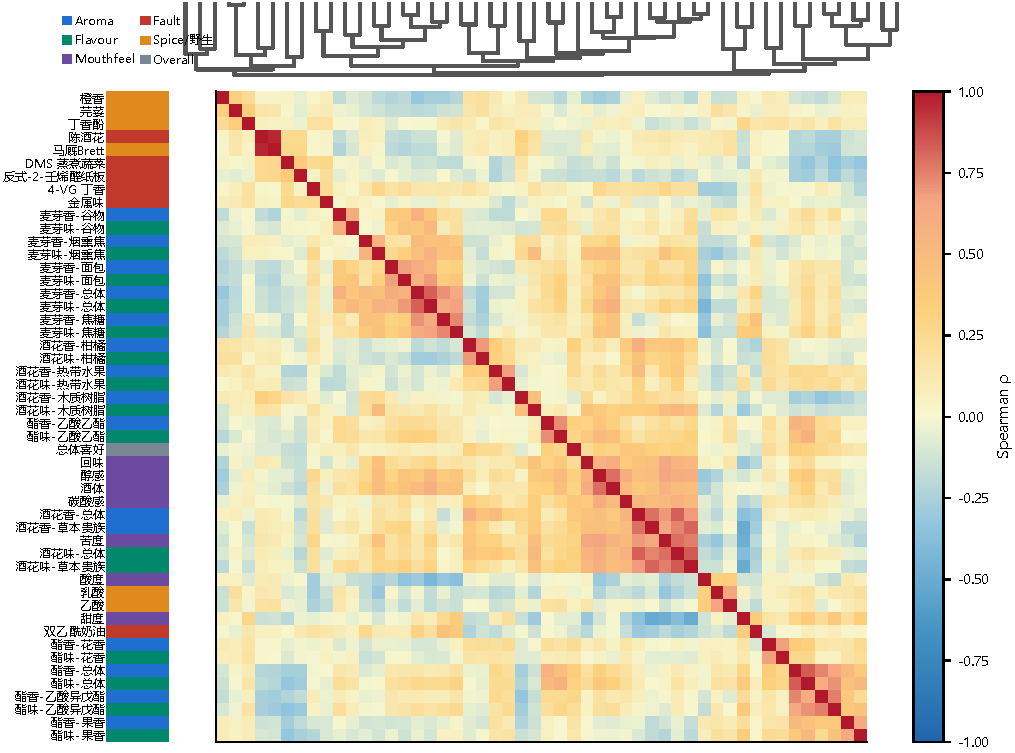
\includegraphics[width=\figw]{images/fig02_sensory_corr.pdf}
\caption{50 个感官维度的 Spearman 相关结构（层次聚类排序）：Aroma 与 Flavour
两套各自成块、同族强相关，缺陷维度与酯香/酒花维度负相关}
\label{fig:sensory}
\end{figure}

\textbf{化学侧}：取 $|\rho|\ge0.3$ 为边，\texttt{2.csv} 构成含 \textbf{4033 条边}、
平均度 34.9 的共表达图；取 $|\rho|\ge0.45$ 并做力导向布局后
（图~\ref{fig:network}），网络清晰分裂为酯类模块、萜烯类模块与醇/酸/硫模块。
模块的化学类别构成（图~\ref{fig:network}(b)）显示：模块 M1 以酯类为主、M2 以萜烯
为主，说明共表达结构主要反映\textbf{代谢通路来源}（乙酸酯类共用乙酰辅酶 A 前体、
萜类共用甲羟戊酸/MEP 途径），而非随机噪声。这一结论是问题二“化学合理性”的
先验基础：若某感官的 Top-3 落在同一模块，其可信度高于三个跨模块的孤立化合物。

上述块状结构可以定量刻画，而不必只依赖热图的目视。记第 $k$ 与第 $k'$ 个感官维度
的 Spearman 相关为 $\rho_{kk'}$，把全部 $\binom{50}{2}=1225$ 个维度对按是否属于
同一感官分组分成两组，分别求平均绝对相关：
\begin{equation}
\bar\rho_{\mathrm{in}}=\frac{1}{|\mathcal{P}_{\mathrm{in}}|}
\sum_{(k,k')\in\mathcal{P}_{\mathrm{in}}}\left|\rho_{kk'}\right|,\qquad
\bar\rho_{\mathrm{out}}=\frac{1}{|\mathcal{P}_{\mathrm{out}}|}
\sum_{(k,k')\in\mathcal{P}_{\mathrm{out}}}\left|\rho_{kk'}\right|,
\label{eq:blockrho}
\end{equation}
其中 $\mathcal{P}_{\mathrm{in}}$ 为同组维度对（261 对），
$\mathcal{P}_{\mathrm{out}}$ 为跨组维度对（964 对）。实测
$\bar\rho_{\mathrm{in}}=0.204$、$\bar\rho_{\mathrm{out}}=0.161$，即\textbf{块内关联
强度是块间的 1.27 倍}；若两组本该无差别，这一比值应接近 1。分组的组内平均相关
差异很大：口感组（Mouthfeel，7 维）最高，达 $0.378$，说明“酒体、醇感、碳酸感、
回味”在品评员的认知中高度耦合、难以独立打分；Aroma 与 Flavour 分别为 $0.180$
与 $0.202$；缺陷组最低（$0.162$），反映缺陷的发生是零散事件而非系统维度。

最强的一对是“陈酒花”与“马厩 Brett”（$\rho=0.966$）。二者在多数样品上同时
缺失、只在少数野生菌参与的样品上同时出现，属于典型的\textbf{共同缺失型伪相关}——
这提醒后续归因不能把共现直接当作因果，也正是问题二要用五路证据而非单一相关系数
做归因的原因之一。

\begin{figure}[H]
\centering
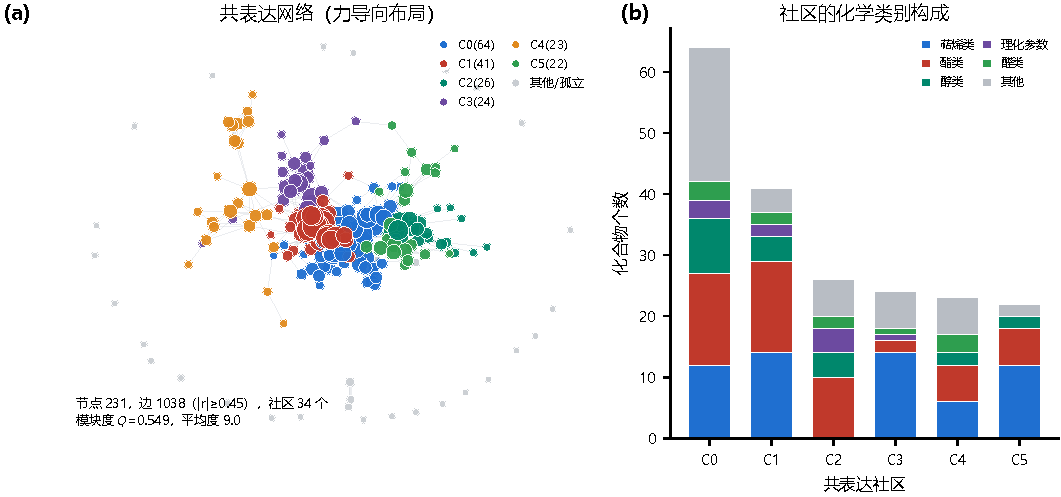
\includegraphics[width=\figw]{images/fig03_compound_network.pdf}
\caption{化合物共表达图：(a) 力导向布局，节点大小表示度、颜色表示共表达模块；
(b) 各模块的化学类别构成，酯类与萜类分别主导不同模块}
\label{fig:network}
\end{figure}

\subsection{气味阈值、来源标注与 OAV}

\texttt{8.xlsx} 的阈值表给出 261 条化合物的来源（Malt / Hops / Yeast / Wild
flora / Spices / Others）、气味阈值与异味描述，其中与 \texttt{1.csv} 可匹配者 47
条、含可用阈值者 \textbf{43 条}、显式标注“异味”者 7 条（乙醛、二乙基硫、DMS、
硫化氢、甲硫醇、双乙酰、SO$_2$）。结合 \S\ref{sec:logbase} 的逐列量纲判定，本文
对 \textbf{41 个化合物}计算了 OAV，结果符合酿造学常识：里那醇
（$\mathrm{OAV}$ 中位数 13.6）、香茅醇 8.8、香叶醇 4.4 等萜烯类长期处于阈值以上
（这解释了为何酒花香是商业啤酒的主导香气）；DMS 中位数 1.41、双乙酰 0.95，
恰在阈值附近浮动，说明缺陷是“少数样品的越界”而非普遍现象
（DMS 有 67.2\% 的样品 $\mathrm{OAV}>1$，双乙酰 44.8\%，4VG 仅 6.4\%）。

OAV 的计算必须建立在 \S\ref{sec:logbase} 的逐列量纲判定之上，否则超痕量致香物会
被系统性高估。正式地，对第 $i$ 个样品的第 $c$ 个化合物，
\begin{equation}
\mathrm{OAV}_{ic}=\frac{C_{ic}}{T_c},\qquad
C_{ic}=
\begin{cases}
10^{\,v_{ic}}, & c\in\mathcal{L}_{\log},\\[2pt]
v_{ic}, & c\in\mathcal{L}_{\mathrm{raw}},
\end{cases}
\label{eq:oav}
\end{equation}
其中 $v_{ic}$ 为 \texttt{1.csv} 中的原始数值，$\mathcal{L}_{\log}$ 与
$\mathcal{L}_{\mathrm{raw}}$ 分别为对数变换列与原始浓度列（由
\S\ref{sec:logbase} 逐列判定），$T_c$ 为气味阈值。表~\ref{tab:oav} 列出 OAV 中位数
最高的 10 个化合物：里那醇、香茅醇、香叶醇三种萜烯醇的 OAV 中位数分别为 13.58、
8.79、4.38，且分别有 98.4\%、92.4\%、76.0\% 的样品超过阈值，说明\textbf{酒花香是
商业啤酒最稳定的可感知香气}；异戊醇乙酸酯（3.62）与乙酸乙酯（1.15）反映酯香；
DMS 与硫化氢代表硫代谢；乙酸来自野生菌群。41 个可算 OAV 的化合物中，有 12 个的
$\mathrm{OAV}>1$ 样品占比超过半数——这一比例说明\textbf{真正的“常驻香气”只占少数}，
多数化合物处于阈值附近，其感官贡献依赖于基质与协同效应，这正是单一 OAV 不足以
解释风味、必须建模的物理原因。

\begin{table}[H]
\centering
\caption{气味活度值（OAV）中位数最高的 10 个化合物}
\label{tab:oav}
\small
\begin{fittable}
\begin{tabular}{@{}lrrrlr@{}}
\toprule
化合物 & 阈值 $T_c$ & 单位 & 来源 & OAV 中位数 & $\mathrm{OAV}>1$ 占比 \\
\midrule
里那醇 Linalool & 0.027 & mg/L & Hops & 13.58 & 98.4\% \\
香茅醇 Citronellol & 0.025 & mg/L & Hops & 8.79 & 92.4\% \\
蛋白质 Protein & 1.024 & g/L & Others & 7.33 & 99.6\% \\
香叶醇 Geraniol & 0.032 & mg/L & Hops & 4.38 & 76.0\% \\
氨 Ammonia & 2.600 & mg/L & Malt & 3.68 & 87.6\% \\
乙酸异戊酯 & 0.603 & mg/L & Yeast & 3.62 & 84.4\% \\
硫化氢 H$_2$S & 3.500 & $\mu$g/L & Yeast & 2.43 & 92.0\% \\
二甲基硫 DMS & 17.250 & $\mu$g/L & Malt & 1.41 & 67.2\% \\
乙酸 Acetic acid & 0.140 & g/L & Wild flora & 1.21 & 61.6\% \\
乙酸乙酯 Ethyl acetate & 24.000 & mg/L & Yeast & 1.15 & 65.6\% \\
\bottomrule
\end{tabular}
\end{fittable}
\end{table}

\begin{figure}[H]
\centering
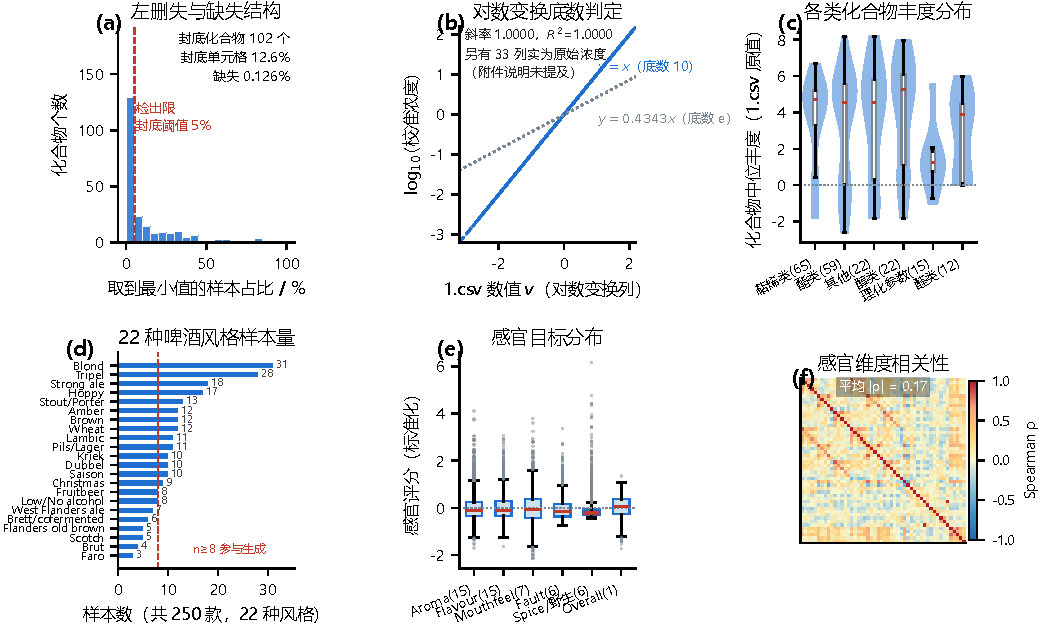
\includegraphics[width=\figw]{images/fig01_data_overview.pdf}
\caption{数据审计六联图：(a) 检出限封底比例分布；(b) 对数底数判定（散点严格落在
$y=x$ 上，33 列为原始浓度）；(c) 各类化合物丰度分布；(d) 22 种风格样本量；
(e) 50 维感官目标分布；(f) 感官维度相关矩阵}
\label{fig:data}
\end{figure}

本节的所有判定（底数 10、33 列原始浓度、102 列封底、0--6 标定、231 双射映射、
41 个 OAV）均由 \texttt{src/01\_audit.py} 一次运行复算，输出 \texttt{audit\_report.txt}
与 \texttt{prepared.npz}，供后续三问共享。
